\documentclass[fleqn]{article}

\usepackage{listings}
\usepackage{diagbox}
\usepackage[german]{babel}
\usepackage[T1]{fontenc}
\usepackage[latin1]{inputenc}
\usepackage{titlesec}
\usepackage{geometry}
\usepackage{qtree}
\usepackage{tikz}
\usepackage{amsmath}
\usepackage{amssymb}
\setcounter{secnumdepth}{0}
\usetikzlibrary{positioning}
\geometry{top=2.5cm, bottom=2.5cm}
\lstset{
 columns=fixed,       
 numbers=left,                                        % 在左侧显示行号
 numberstyle=\tiny\color{gray},                       % 设定行号格式
 frame=none,                                          % 不显示背景边框
 backgroundcolor=\color[RGB]{245,245,244},            % 设定背景颜色
 keywordstyle=\color[RGB]{40,40,255},                 % 设定关键字颜色
 numberstyle=\footnotesize\color{darkgray},           
 commentstyle=\it\color[RGB]{0,96,96},                % 设置代码注释的格式
 stringstyle=\rmfamily\slshape\color[RGB]{128,0,0},   % 设置字符串格式
 showstringspaces=false,                              % 不显示字符串中的空格
 language=c++,                                        % 设置语言
 breaklines,                                          % 自动换行
}

\title{TU Chemnitz \\ Praktikum Grundlagen Technische Informatik \\ Versuch Komb 2}

\author{Gruppe 5 - Team 5: \\ Dongze Yang \\Xiangyu Tong \\ Treshchun Kateryna}

\begin{document}

\maketitle



\newpagestyle{main}{
    \sethead{}{}{Grupe 5 - Team 5}
    \setfoot{}{\thepage}{}
    \headrule
    \footrule
}
\pagestyle{main}
%\section{Aufgabe}

$$y = (a,b,c,d) = ab\overline{c}\vee acd \vee \bar{a}\bar{c}d \vee \overline{a}\overline{b}c$$

\textbf{Wahrheitstabelle:}

\begin{center}
\begin{tabular}{cccc|c}
    $a$ & $b$ & $c$ & $d$ & $y$\\
    \hline
    0&0&0&0&0\\
    0&0&0&1&1\\
    0&0&1&0&1\\
    0&0&1&1&1\\
    \hline
    0&1&0&0&0\\
    0&1&0&1&1\\
    0&1&1&0&0\\
    0&1&1&1&0\\
    \hline
    1&0&0&0&0\\
    1&0&0&1&0\\
    1&0&1&0&0\\
    1&0&1&1&1\\
    \hline
    1&1&0&0&1\\
    1&1&0&1&1\\
    1&1&1&0&0\\
    1&1&1&1&1\\
\end{tabular}
\end{center}

\textbf{8-zu-1-Multiplexer:}

\begin{equation}
\begin{aligned}
 y =& \bar{a}\bar{b}\bar{c}\bar{d}0 + \bar{a}\bar{b}\bar{c}d1 + \bar{a}\bar{b}c\bar{d}1 + \bar{a}\bar{b}cd1 +
 \bar{a}b\bar{c}\bar{d}0 + \bar{a}b\bar{c}d1 + \bar{a}bc\bar{d}0 + \bar{a}bcd0+\\
 &a\bar{b}\bar{c}\bar{d}0 + a\bar{b}\bar{c}d0 + a\bar{b}c\bar{d}0 + a\bar{b}cd1+
 ab\bar{c}\bar{d}1 + ab\bar{c}d1 + abc\bar{d}0 + abcd1\\
 =&\bar{a}\bar{b}\bar{c}(\bar{d}0+d1) + \bar{a}\bar{b}c(\bar{d}1+d1) + \bar{a}b\bar{c}(\bar{d}0+d1) + \bar{a}bc(\bar{d}0+d0)+\\
 &a\bar{b}\bar{c}(\bar{d}0+d0) + a\bar{b}c(\bar{d}0+d1)+ ab\bar{c}(\bar{d}1+d1)+abc(\bar{d}0+d1)\\
 \\
 g =&\bar{s_2}\bar{s_1}\bar{s_0}d+\bar{s_2}\bar{s_1}s_01+\bar{s_2}s_1\bar{s_0}d+\bar{s_2}s_1s_00+\\
 &s_2\bar{s_1}\bar{s_0}0+s_2\bar{s_1}s_0d+s_2s_1\bar{s_0}1+s_2s_1s_0d\\
 \\
 & d_0 = d_2 = d_5 = d_7 = d ,\, d_1 = d_6 = 1,\, d_3 = d_4 = 0
\end{aligned}
\end{equation}

\textbf{4-zu-1-Multiplexer:}

\begin{equation}
    \begin{aligned}
        y =& \bar{a}\bar{b}(\bar{c}\bar{d}0+\bar{c}d1+c\bar{d}1+cd1) + \bar{a}b(\bar{c}\bar{d}0+\bar{c}d1+c\bar{d}0+cd0)+\\
        &a\bar{b}(\bar{c}\bar{d}0+\bar{c}d0+c\bar{d}0+cd1)+ ab(\bar{c}\bar{d}1+\bar{c}d1+c\bar{d}0+cd1)\\
        =& \bar{a}\bar{b}(\overline{\bar{c}\bar{d}}) + \bar{a}b(\bar{c}d) + a\bar{b}(cd) + ab(\overline{c\bar{d}})\\
        \\
        g=& \bar{s_1}\bar{s_0}(\overline{\bar{c}\bar{d}}) + \bar{s_1}s_0(\bar{c}d) + s_1\bar{s_0}(cd) + s_1s_0(\overline{c\bar{d}})\\
        \\
        &d_0=\overline{\bar{c}\bar{d}},\, d_1=\bar{c}d,\, d_2=cd ,\, d_3=\overline{c\bar{d}}
    \end{aligned}
\end{equation}


\textbf{Schaltplan der Realisierung}

\begin{figure}[htbp]
\centering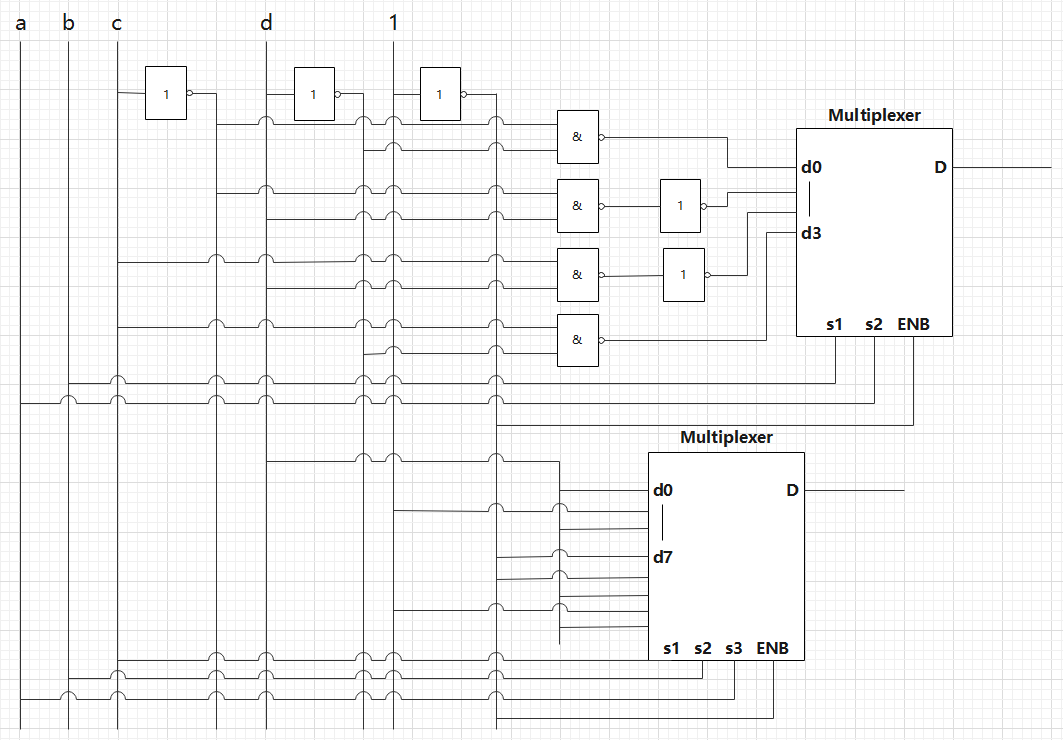
\includegraphics[width=6in]{bild1.png}
\caption{Schaltbild}
\end{figure}

\textbf{VHDL-Strukturbeschreibung}
 
\begin{lstlisting}
    library ieee; 
    use ieee.std_logic_1164.all; 
    use work.pack_2.all;
    entity uut is 
            port ( EE_X : in x01_vector(7 downto 0); 
                EE_Y : out x01_vector(23 downto 16) ); 
    end uut;
    
    architecture structure of uut is
      alias a  : x01 is EE_X(0);
      alias b  : x01 is EE_X(1);
      alias c  : x01 is EE_X(2);
      alias d  : x01 is EE_X(3);
    
    
        component sn7400 is -- 2er NAND 
            port ( x : in X01_vector (1 to 2); 
                y : out X01 ); 
        end component;
    
        component sn7404 is -- Negatoren 
            port ( x : in X01; 
                y : out X01 ); 
        end component;
    
        component sn74151 is -- 8zu1 Multiplexer 
            port ( e : in X01; 
                s : in X01_vector (2 downto 0); 
                d : in X01_vector (0 to 7); 
                y,w : out X01 ); 
        end component;
        
        component sn74153 is -- 4zu1 Multiplexer 
            port ( e1,e2 : in X01; 
                s : in X01_vector (1 downto 0); 
                d1,d2 : in X01_vector (0 to 3); 
                y1,y2 : out X01 );
        end component;
    
        signal not_a,not_b,not_c,not_d : X01; 
        signal md0, md1, md2, md3 : X01; 
        signal buffy0 ,buffy1 : X01;
    
    begin
        -- Block 1: Negation
        NOTA: sn7404 port map(x=>a, y=>not_a);
        NOTB: sn7404 port map(x=>b, y=>not_b); 
        NOTC: sn7404 port map(x=>c, y=>not_c); 
        NOTD: sn7404 port map(x=>d, y=>not_d);
        TEMP0: sn7400 port map(x(1)=>not_c, x(2)=>not_d, y=>md0); 
        TEMP1_0: sn7400 port map(x(1)=>not_c, x(2)=>d, y=>buffy0); 
        TEMP1_1: sn7404 port map(x=>buffy0 ,y=>md1);
        TEMP2_0: sn7400 port map(x(1)=>c,x(2)=>d,y=>buffy1);
        TEMP2_1: sn7404 port map(x=>buffy1 ,y=>md2);
        TEMP3_1: sn7400 port map(x(1)=>c,x(2)=>not_d,y=>md3);
        -- Block 2: 8-zu-1-Multiplexer
        MULTI8: sn74151 port map ( e => '0',
                                s(2)=>a, s(1)=>b, s(0)=>c,
                                d(0)=>d, d(1)=>'1', d(2)=>d, d(3)=>'0', 
                                d(4)=>'0', d(5)=>d, d(6)=>'1', d(7)=>d,
                                y=>EE_Y(16)
                                );
        -- Block 3: 4-zu-1-Multiplexer
        MULTI4: sn74153 port map ( e1 => '0', e2 =>'1',
                                s(1) => a, s(0) => b,
                                d1(0) => md0, d1(1) => md1, d1(2) => md2, d1(3) => md3,
                                d2(0) => '0', d2(1) => '0', d2(2) => '0', d2(3) => '0',
                                y1 => EE_Y(17)
                                );
    end structure;

\end{lstlisting}



\textbf{binäre Stimulusfolge}
\begin{lstlisting}
stimmap dbb2_08 0000----|00-----
stimmap dbb2_08 0001----|11-----
stimmap dbb2_08 0011----|11-----
stimmap dbb2_08 0010----|11-----
stimmap dbb2_08 0110----|00-----
stimmap dbb2_08 0111----|00-----
stimmap dbb2_08 0101----|11-----
stimmap dbb2_08 0100----|00-----
stimmap dbb2_08 1100----|11-----
stimmap dbb2_08 1101----|11-----
stimmap dbb2_08 1111----|11-----
stimmap dbb2_08 1110----|00-----
stimmap dbb2_08 1010----|00-----
stimmap dbb2_08 1011----|11-----
stimmap dbb2_08 1001----|00-----
stimmap dbb2_08 1000----|00-----
\end{lstlisting}

\textbf{Simulation}
\begin{lstlisting}
1 0000---- -> 00XXXXXX                                         
              00----- 
                     ^
2 0001---- -> 11XXXXXX                                         
              11----- 
                     ^
3 0011---- -> 11XXXXXX                                         
              11----- 
                     ^
4 0010---- -> 11XXXXXX                                         
              11----- 
                     ^
5 0110---- -> 00XXXXXX                                         
              00----- 
                     ^
6 0111---- -> 00XXXXXX                                         
              00----- 
                     ^
7 0101---- -> 11XXXXXX                                         
              11----- 
                     ^
8 0100---- -> 00XXXXXX                                         
              00----- 
                     ^
9 1100---- -> 11XXXXXX                                         
              11----- 
                     ^
10 1101---- -> 11XXXXXX                                         
               11----- 
                      ^
11 1111---- -> 11XXXXXX                                         
               11----- 
                      ^
12 1110---- -> 00XXXXXX                                         
               00----- 
                      ^
13 1010---- -> 00XXXXXX                                         
               00----- 
                      ^
14 1011---- -> 11XXXXXX                                         
               11----- 
                      ^
15 1001---- -> 00XXXXXX                                         
               00----- 
                      ^
16 1000---- -> 00XXXXXX                                         
               00----- 
                     ^
\end{lstlisting}

% Aufgabe 2
\textbf{binäre Stimulusfolge minimaler Länge}

\begin{figure}[htbp]
    \centering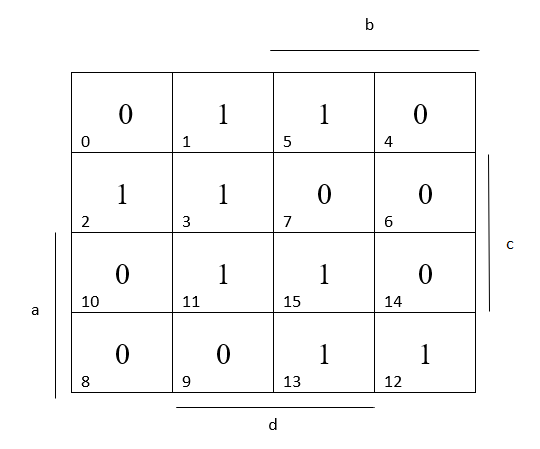
\includegraphics[width=5in]{bild2.png}
    \caption{Karnaugh-Veitch-Diagramm}
\end{figure}

\begin{equation}
    \begin{aligned}
&f|_{a=0} \nsim f|_{a=1} = \bar{b}c\bar{d}+\bar{b}\bar{c}d+bcd+b\bar{c}\bar{d}\\
&\Rightarrow T_{a\equiv 0}(a,b,c,d) = (1,0,1,0)|(1,0,0,1)|(1,1,1,1)|(1,1,0,0)\\
&\Rightarrow T_{a\equiv 1}(a,b,c,d) = (0,0,1,0)|(0,0,0,1)|(0,1,1,1)|(0,1,0,0)
    \end{aligned}
\end{equation}

\begin{equation}
    \begin{aligned}
&f|_{b=0} \nsim f|_{b=1} = \bar{a}cd+\bar{a}c\bar{d}+a\bar{c}d+a\bar{c}\bar{d}\\
&\Rightarrow T_{b\equiv 0}(a,b,c,d) = (0,1,1,1)|(0,1,1,0)|(1,1,0,1)|(1,1,0,0)\\
&\Rightarrow T_{b\equiv 1}(a,b,c,d) = (0,0,1,1)|(0,0,1,0)|(1,0,0,1)|(1,0,0,0)
    \end{aligned}
\end{equation}

\begin{equation}
    \begin{aligned}
&f|_{c=0} \nsim f|_{c=1} = \bar{a}\bar{b}\bar{d}+a\bar{b}d+\bar{a}db+ab\bar{d}\\
&\Rightarrow T_{c\equiv 0}(a,b,c,d) = (0,0,1,0)|(1,0,1,1)|(0,1,1,1)|(1,1,1,0)\\
&\Rightarrow T_{c\equiv 1}(a,b,c,d) = (0,0,0,0)|(1,0,0,1)|(0,1,0,1)|(1,1,0,0)
    \end{aligned}
\end{equation}

\begin{equation}
    \begin{aligned}
&f|_{d=0} \nsim f|_{d=1} =  \bar{a}\bar{b}\bar{c}+\bar{a}b\bar{c}+a\bar{b}c+abc\\
&\Rightarrow T_{d\equiv 0}(a,b,c,d) = (0,0,0,1)|(0,1,0,1)|(1,0,1,1)|(1,1,1,1)\\
&\Rightarrow T_{d\equiv 1}(a,b,c,d) = (0,0,0,0)|(0,1,0,0)|(1,0,1,0)|(1,1,1,0)
    \end{aligned}
\end{equation}

\begin{equation}
    \begin{aligned}
T_{y\equiv0} = \bar{a}\bar{b}\bar{c}d+\bar{a}\bar{b}c\bar{d}+\bar{a}\bar{b}cd+\bar{a}b\bar{c}d+a\bar{b}cd+ab\bar{c}\bar{d}+ab\bar{c}d+abcd\\
\Rightarrow T_{y\equiv 0}(a,b,c,d) = (0,0,0,1)|(0,0,1,0)|(0,0,1,1)|(0,1,0,1)|\\(1,0,1,1)|(1,1,0,0)|(1,1,0,1)|(1,1,1,1)\\
T_{y\equiv1} = \bar{a}\bar{b}\bar{c}\bar{d}+\bar{a}b\bar{c}\bar{d}+\bar{a}bc\bar{d}+\bar{a}bcd+a\bar{b}\bar{c}\bar{d}+a\bar{b}\bar{c}d+a\bar{b}c\bar{d}+abc\bar{d}\\
\Rightarrow T_{y\equiv 1}(a,b,c,d) = (0,0,0,0)|(0,1,0,0)|(0,1,1,0)|(0,1,1,1)|\\(1,0,0,0)|(1,0,0,1)|(1,0,1,0)|(1,1,1,0)
    \end{aligned}
\end{equation}

\textbf{Überdeckungen}

\begin{center}
    \begin{tabular}{|c|c|c|c|c|c|c|c|c|c|c|c|}
        \hline
        abcd&a=0&a=1&b=0&b=1&c=0&c=1&d=0&d=1&y=0&y=1&Ergebnis\\
        \hline
        0000&&&&&&1&&1&&1&\\
        \hline
        0001&&1&&&&&1&&1&&\\
        \hline
        0010&&1&&1&1&&&&1&&$\Leftarrow$\\
        \hline
        0011&&&&1&&&&&1&&\\
        \hline
        0100&&1&&&&&&1&&1&\\
        \hline
        0101&&&&&&1&1&&1&&\\
        \hline
        0110&&&1&&&&&&&1&\\
        \hline
        0111&&1&1&&1&&&&&1&$\Leftarrow$\\
        \hline
        1000&&&&1&&&&&&1&\\
        \hline
        1001&1&&&1&&1&&&&1&$\Leftarrow$\\
        \hline
        1010&1&&&&&&&1&&1&\\
        \hline
        1011&&&&&1&&1&&1&&\\
        \hline
        1100&1&&1&&&1&&&1&&$\Leftarrow$\\
        \hline
        1101&&&1&&&&&&1&&\\
        \hline
        1110&&&&&1&&&1&&1&\\
        \hline
        1111&1&&&&&&1&&1&&\\
        \hline
    \end{tabular}
\end{center}

\textbf{Stimulus}

\begin{lstlisting}
stimmap dbb2_08 0010----|11------
stimmap dbb2_08 0111----|00------
stimmap dbb2_08 1001----|00------
stimmap dbb2_08 1100----|11------
\end{lstlisting}

\end{document}